\chapter{Theoretical Foundations} \label{chap:theoretical-foundations}
This chapter gives a brief insight into the mathematical and experimental foundations regarding electron holography and tomography, solid state physics as well as numerical modeling and simulation of semiconductor nanostructures.
\section{Solid State Physics} \label{sec:solid-state-physics}
Despite the study of solids and their physical properties having a rich scientific history, modern solid state physics did not emerge until the 20\textsuperscript{th}~century, ultimately culminating in the invention of the transistor in 1947 and the integrated circuit in 1958, which marked the beginning the of the information age and changed the world like hardly any other invention \cite{Alferov1998,Jenkins2005,Lukasiak2010,Klein2016}. Therefore, the following \cref{ssec:blochs-theorem,ssec:density-of-states-doping,ssec:band-structure-p-n-junctions} provide a concise description of $p$-$n$-junction semiconductors from a solid state physics perspective.
\subsection{Bloch's Theorem} \label{ssec:blochs-theorem}
Crystalline solids are characterized by their periodic structure, resulting in the formation of continuous energy bands that arise from the discrete electronic states within these solids \cite{Kittel1987,Piprek2003,Yu2010}. In such many-body electron systems, the Hamiltonian is given by:
\begin{equation}
  H = \sum_i \left[ \frac{\vb{p}_i^2}{2m_0} + V_{\mathit{ion}}\left(\vb{r}_i\right) \right] + \frac{1}{2} \sum_{i \neq j} \frac{e^2}{4\pi |\vb{r}_i - \vb{r}_j|},
\end{equation}
where $\vb{p}_i^2 / 2m_0$ represents the electrons kinetic energy, $V_{\mathit{ion}}\left(\vb{r}_i\right)$ the electron-core interaction energy and the last sum the Coulomb interaction energy between electrons \cite{Kittel1987,Piprek2003,Yu2010}.

Solving this type of Hamiltonian for systems as large as electronic ensembles in solids becomes unfeasible, requiring the introduction of an effective one-body Hamiltonian:
\begin{equation}
H = \frac{\vb{p}^2}{2m_0} + V_{\mathit{ion}}\left(\vb{r}\right) + V\left[n_0\right]\left(\vb{r}\right),
\end{equation}
where the one-body potential energy $V\left[n_0\right]\left(\vb{r}\right)$ replaces the electron-electron interaction energy and is a functional of the ground state electron density $n_0$\footnote{In 1964, Walter Kohn and Pierre Claude Hohenberg proved that the ground state properties of a many-electron system are a unique functional of the ground state electron density, therefore established the Hohenberg-Kohn theorem as the foundation for density functional theory \cite{Hohenberg1964}.} of the effective one-body Hamiltonian:
\begin{equation}
  n_0\left(\vb{r}\right) = \sum_{E_n < E_F} |\psi_n\left(\vb{r}\right)|^2 \quad ; \quad H\psi_n = E_n\psi_n,
\end{equation}
with the eigenfunctions $\psi_n$ of the effective one-body Hamiltonian $H$ and their corresponding energies $E_n$\footnote{The Pauli exclusion principle states that every eigenstate $n$ can only be occupied by a maximum of two electrons with opposite spin \cite{Kittel1987,Kittel2004,Yu2010}.} \cite{Kittel1987,Piprek2003,Yu2010}.

The eigenfunctions $\psi_n$ form a plane wave modulated by a periodic function according to Bloch's theorem:
\begin{equation}
  \label{eq:bloch-theorem}
  \psi_{n,\vb{k}}\left(\vb{r}\right) = u_{n,\vb{k}}\left(\vb{r}\right) e^{i\vb{k} \cdot \vb{r}},
\end{equation}
with the wave vector $\vb{k}$ and a periodic function $u_{n,\vb{k}}\left(\vb{r}\right)$ \cite{Kittel1987,Piprek2003,Yu2010}.

While the formation of continuous energy bands is not exclusive to certain types of solids, the binary occupation (either fully occupied or empty) of each band in the ground state is a distinctive characteristic of semiconductors, where the highest occupied energy band (i.\,e.\ the valence band) and the lowest energy unoccupied band (i.\,e.\ the conduction band) are separated by a band gap $E_G$, with the Fermi energy $E_F$ lying in between them \cite{Kittel1987,Piprek2003,Yu2010}.
\subsection{Density of States and Doping} \label{ssec:density-of-states-doping}
Assuming a non-interacting many-electron system, the probability that an electron will occupy a given band state in thermodynamic equilibrium with energy $E$ is given by the Fermi-Dirac distribution function:
\begin{equation}
  f\left(E\right) = \frac{1}{1 + e^{\frac{E-\mu_F}{k_B T}}},
\end{equation}
where $k_B$ is the Boltzmann constant and $\mu_F$ the chemical potential \cite{Piprek2003,Kittel2004,Yu2010}. At absolute zero, i.\,e.\ $T = \SI{0}{\kelvin}$, the chemical potential~$\mu_F$ is equivalent to the Fermi energy~$E_F$, which corresponds to the highest electron energy \cite{Piprek2003,Kittel2004,Yu2010}. For rising temperatures, the transfer of electrons from the valence band to the conduction band increases, yielding the density of states for both electron bands:
\begin{alignat}{3}
  D_C\left(E\right) &= \frac{1}{2\pi^2} \left(\frac{2m_C^\ast}{\hbar^2}\right)^{3/2} \sqrt{E-E_C} &\qquad\text{Conduction Band $\left(E > E_C\right)$}&\\
  D_V\left(E\right) &= \frac{1}{2\pi^2} \left(\frac{2m_V^\ast}{\hbar^2}\right)^{3/2} \sqrt{E_V-E} &\qquad\text{Valence Band $\left(E<E_V\right)$}&,
\end{alignat}

with the effective masses of electrons and holes $m_C^\ast$ and $m_V^\ast$, the lower edge conduction band energy~$E_C$ and the upper edge valence band energy~$E_V$ \cite{Piprek2003,Kittel2004,Yu2010}.

For the case where the Fermi~energy is separated from the electron band by more than $3k_B T$, the associated semiconductor is considered non-degenerate and intrinsic, resulting in substandard electrical conductivity at room temperature \cite{Piprek2003,Kittel2004,Yu2010}. This inferior suitability of intrinsic semiconductors for electrical circuits raises the need for the increase of the electrical conductivity of such semiconductors through doping (i.\,e.\ the intentional introduction of impurity atoms) \cite{Piprek2003,Kittel2004,Yu2010}. These donor and acceptor atoms create energy states close to the lower edge conduction band energy~$E_C$ (i.\,e.\ $n$-doping) and upper edge valence band energy~$E_V$ (i.\,e.\ $p$-doping), thereby releasing an electron into the conduction band or creating a hole through the acceptance of an electron from the valence band \cite{Piprek2003,Kittel2004,Yu2010}. Doped semiconductors therefore become degenerate, subsequently making their majority charge carrier concentration considerably greater than their minority carrier concentration \cite{Piprek2003,Kittel2004,Yu2010}.
\subsection[Electron Band Structure of \texorpdfstring{$p$-$n$}{\textit{p}-\textit{n}}-Junctions]{Electron Band Structure of $\boldsymbol{p}$-$\boldsymbol{n}$-Junctions} \label{ssec:band-structure-p-n-junctions}
One of the fundamental building blocks of electrical circuits are diodes based on the $p$-$n$-junction, a boundary between a $p$-doped and $n$-doped semiconductor that acts as a passthrough for the current in one direction (i.\,e.\ forward bias) while allowing little to no current flow in the opposite direction (i.\,e.\ reverse bias) \cite{Hook1991,Piprek2003,Kittel2004}. In thermal equilibrium, holes from the $p$-side and electrons from the $n$-side diffuse into the opposite region, where they recombine and create a depletion region, leaving behind a surplus of ionized charge carriers that create an electric field to offset the charge carrier diffusion \cite{Hook1991,Piprek2003,Kittel2004}. At equilibrium (i.\,e.\ without an external bias) the Fermi-energy $E_F$ is represented by a flat line and a potential difference (i.\,e.\ the built-in potential $\phi_{\mathit{bi}}$) forms across the junction, where the 1D~electric field and charge carrier density are obtained by the first- and second-order derivative (\cref{fig:p-n-junction-potential-efield-charge-carrier-density}), yielding:
\begin{equation}
  \label{eq:pn-junction-potential}
  \phi\left(r\right) =
  \begin{dcases}
    \frac{e N_A\left(r\right)}{2\epsilon\left(r\right) }\left(r + \omega_p\right)^2  & -\omega_p < r < 0 \\
    \Delta \phi_0 - \frac{e N_D\left(r\right)}{2\epsilon\left(r\right) }\left(r - \omega_n\right)^2 & \phantom{-}0 < r < \omega_n,
  \end{dcases}
\end{equation}
with the dielectric tensor $\epsilon\left(r\right) = \epsilon_0 \epsilon_r \left(r\right)$, where $\epsilon_0$ is the vacuum permittivity, the donor and acceptor atom density $N_D\left(r\right)$ and $N_A\left(r\right)$ and the potential difference $\phi_0 = e / 2 \epsilon\left(r\right)  \left(N_A\left(r\right) \omega_p^2 + N_D\left(r\right) \omega_n^2\right)$ that is continuous at $r = 0$, from which ultimately the widths of the depletion region follow \cite{Hook1991,Piprek2003,Kittel2004}:
\begin{align}
  \omega_n &= \left(\frac{2 \epsilon\left(r\right)  N_A\left(r\right) \Delta \phi_0}{e N_D\left(r\right) \left(N_A\left(r\right) + N_D\left(r\right)\right)}\right)^{1/2} \label{eq:depletion-region-width-n-region} \\
   \omega_p &= \left(\frac{2 \epsilon\left(r\right)  N_D\left(r\right) \Delta \phi_0}{e N_A\left(r\right) \left(N_A\left(r\right) + N_D\left(r\right)\right)}\right)^{1/2}. \label{eq:depletion-region-width-p-region}
\end{align}
By applying a forward bias $V$, i.\,e.\ connecting the positive terminal with the $p$-side and the negative terminal with the $n$-side, the potential difference $\Delta \phi = \Delta \phi_0 - V$ decreases and the constant flow of majority charge carriers on each side of the diode causes the depletion region to decrease as well \cite{Hook1991,Piprek2003,Kittel2004}. Furthermore, applying a forward bias causes the energy levels of the minority charge carriers on the $p$-side (i.\,e.\ the electrons) to be lowered relative to the majority charge carriers on the $n$-side, therefore shrinking the energy barrier and increasing the electron flow from the $n$-side to the $p$-side \cite{Hook1991,Piprek2003,Kittel2004}.
\begin{figure}[H]
	\centering
	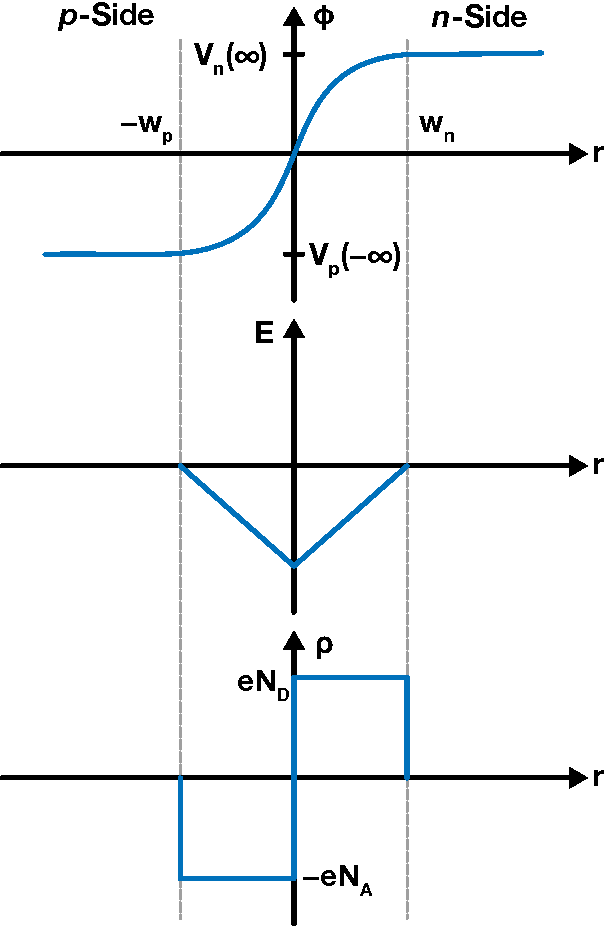
\includegraphics[width=0.5\textwidth]{Figures/Schematics/Theoretical Foundations/p-n-junction-potential-efield-charge-carrier-density.pdf}
	\caption{Schematic illustration of the electrostatic potential $\phi\left(r\right)$, the electric field $E\left(r\right)$ and the charge carrier density $\rho\left(r\right)$ across a $p$-$n$-junction, where the dashed lines indicate the width of the depletion region from $-w_p$ to $w_n$ \cite{Hook1991,Piprek2003,Kittel2004}.}
	\label{fig:p-n-junction-potential-efield-charge-carrier-density}
\end{figure}
This bending of the electron bands can likewise be observed with a reverse bias applied (positive terminal connected to the $n$-side and negative terminal to the $p$-side), where the flow of majority charge carriers across the diode is drastically reduced through the increased potential barrier, effectively minimizing the charge flow \cite{Hook1991,Piprek2003,Kittel2004}.
\section{Numerical Modeling of Semiconductor Nanostructures} \label{sec:nextnano-modeling}
Over the past 50 years, unprecedented technological advances have made large scale modeling and simulation of sophisticated nanoscale structures and electrical circuits computationally and economically viable \cite{More1965,Bank1990,Smith1997,Flamm2003,Wachutka2004,Mack2011,Leiserson2020}. On this basis, the \emph{nextnano} software package\footnote{A software license was graciously provided by Dr.~Stefan Birner for the purpose of this work.} enables the characterization of various physical and optical properties of such nanodevices by solving the Schrödinger-Poisson-current equation and 8-band $\vb{k}\cdot\vb{p}$~model self-consistently \cite{Birner2006,Trellakis2006,Birner2007}, as described in detail in \cref{ssec:k-p-method,ssec:schrödinger-current-poisson-equation,ssec:numerical-approaches}.
\subsection{\boldmath\texorpdfstring{$\vb{k}\cdot\vb{p}$}{k·p} Perturbation Theory} \label{ssec:k-p-method}
While various different methods and approximations for determining the band structure and related physical and optical properties of solids have been developed throughout the years, such as density functional theory \cite{Hellmann1935,Hohenberg1964,Kohn1965,Topp1973,Langreth1983,Becke1988,Perdew1992}, Green's functions methods and the Korringa-Kohn-Rostoker method \cite{Korringa1947,Kohn1954,Dupree1961,Morgan1966,Beeby1967,Madelung1967,Zeller1995,Wildberger1997,Papanikolaou2002,Buth2005,Jiang2011}, the tight-binding model \cite{Slater1954,Kwon1994,Lenosky1997,Schulz2005}, dynamic mean field theory \cite{Georges1992,Georges1996,Kotliar2004,Vollhardt2010}, the Kronig-Penney model \cite{Kronig1931,Singh1983,Cho1987,Yuh1988}, or the Hubbard model \cite{Hubbard1963-I,Hubbard1964-II,Hubbard1964-III}, this section focuses on the (multi-band) $\vb{k}\cdot\vb{p}$~method, as used by \emph{nextnano} \cite{Birner2006,Trellakis2006,Birner2007}. One advantage of this approach is that the band structure over the whole Brillouin zone can be extrapolated from the energy of the zone's center, yielding analytical expressions for the band dispersion and effective masses around high symmetry points \cite{Kittel1987,Piprek2003,Yu2010}.

Using the $\vb{k}\cdot\vb{p}$~approximation, the band structure of solids around $\vb{k}_0$\footnote{Usually the $\Gamma$-Point where $\vb{k}_0 = 0$ \cite{Kittel1987,Piprek2003,Yu2010}.}, for which the solution of the Schrödinger equation is known, can be extrapolated by a perturbation theory approach \cite{Kittel1987,Piprek2003,Yu2010}. Inserting the Bloch functions~\labelcref{eq:bloch-theorem} into the single-electron Schrödinger equation yields:
\begin{equation}
  \left[ \frac{p^2}{2m_0} + \frac{\hbar}{m_0}\vb{k}\cdot\vb{p} + eV\left(\vb{r}\right)\right]u_{n,\vb{k}}\left(\vb{r}\right) = \left[E_n\left(\vb{k}\right) - \frac{\hbar^2k^2}{2m_0}\right]u_{n,\vb{k}}\left(\vb{r}\right),
\end{equation}
allowing for the linear expansion of the Bloch functions $u_{n,\vb{k}}\left(\vb{r}\right)$ of the solution $u_{n,\vb{k}_0}\left(\vb{r}\right)$ at the known wave vector $\vb{k}_0$:
\begin{equation}
  u_{n,\vb{k}}\left(\vb{r}\right) = \sum_m a_{n,m} u_{m,\vb{k}_0}\left(\vb{r}\right),
\end{equation}
with the expansion coefficients $a_{n,m}$ \cite{Kittel1987,Piprek2003,Yu2010}. With this, the Hamiltonian can be simplified:
\begin{equation}
  H = H_0 + H_{\vb{k}}',
\end{equation}
with the unperturbated Hamiltonian $H_0$ and the perturbation $H_{\vb{k}}'$, giving the $\vb{k}\cdot\vb{p}$~method its distinctive name \cite{Kittel1987,Piprek2003,Yu2010}.

In the non-degenerate case, the eigenfunctions $u_{n,\vb{k}}\left(\vb{r}\right)$ and eigenvalues $E_{n,\vb{k}}$ can be expanded to second order in $\vb{k}$, yielding:
\begin{align}
  u_{n,\vb{k}}\left(\vb{r}\right) &= u_{n,\vb{k}_0}\left(\vb{r}\right) + \frac{\hbar}{m_0}\sum_{n'\neq n} \frac{\mel**{u_{n,\vb{k}_0}\left(\vb{r}\right)}{\vb{k}\cdot\vb{p}}{u_{n',\vb{k}_0}\left(\vb{r}\right)}}{E_{n,\vb{k}_0} - E_{n',\vb{k}_0}} u_{n',\vb{k}_0} \\
  E_{n,\vb{k}} &= E_{n,\vb{k}_0} + \frac{\hbar^2k^2}{2m_0} + \frac{\hbar^2}{m_0^2}\sum_{n' \neq n} \frac{|\mel**{u_{n,\vb{k}_0}\left(\vb{r}\right)}{\vb{k}\cdot\vb{p}}{u_{n',\vb{k}_0}\left(\vb{r}\right)}|^2}{E_{n,\vb{k}_0} - E_{n',\vb{k}_0}},
\end{align}
where the linear terms in $k$ vanish \cite{Kittel1987,Piprek2003,Yu2010}. The energy $E_{n,\vb{k}}$ can thus be rewritten for small~$k$:
\begin{equation}
  E_{n,\vb{k}} = E_{n,\vb{k}_0} + \frac{\hbar^2k^2}{2_m^\ast},
\end{equation}
from which the effective mass $m^\ast$ can be derived \cite{Kittel1987,Piprek2003,Yu2010}:
\begin{equation}
  \frac{1}{m^\ast} = \frac{1}{m_0} + \frac{1}{m^2k^2} \sum_{n' \neq n} \frac{|\mel**{u_{n,\vb{k}_0}\left(\vb{r}\right)}{\vb{k}\cdot\vb{p}}{u_{n',\vb{k}_0}\left(\vb{r}\right)}|^2}{E_{n,\vb{k}_0} - E_{n',\vb{k}_0}}.
\end{equation}
For a more accurate description of the band structure, it is necessary to consider the spin-orbit interaction, for which the Hamiltonian becomes:
\begin{equation}
  H_k' = \frac{p^2}{2m_0} + \frac{\hbar}{m_0}\vb{k}\cdot\vb{p} + \frac{\hbar^2k^2}{2m_0} + V\left(\vb{r}\right) + \frac{\hbar}{4m_0^2c^2} \left(\grad V\left(\vb{r}\right) \cp \left(\vb{p} + \hbar\vb{k}\right)\right) \cdot \vb{\sigma},
\end{equation}
with the three Pauli matrices $\vb{\sigma} = \left(\sigma_x, \sigma_y, \sigma_z\right)$ \cite{Kittel1987,Piprek2003,Yu2010}.

Separating the electron bands into two groups $A$ and $B$ allows for the derivation of a finite dimensional Hamiltonian \cite{Loewdin1951,Kane1966}, where the number of bands in group $A$ gives rise to the different multi-band $\vb{k}\cdot\vb{p}$~methods \cite{Luttinger1955,Luttinger1956}, with the most commonly used ones being the 4-band\footnote{The 4~bands are: conduction~(C), heavy hole~(HH), light hole~(LH) and split-off~(SO) \cite{Deen2012,Piprek2003}.} method \cite{Deen2012,Piprek2003}, the 6-band method \cite{Chao1992,Zhukov2013} and the 8-band method \cite{Kane1957,Chuang1996,Bahder1990,Enders1995}.
\subsection{Schrödinger-Poisson-Current Equation} \label{ssec:schrödinger-current-poisson-equation}
A description of the electrostatic potential of semiconductors is given by the Poisson equation:
\begin{equation}
  \grad\left[\epsilon\left(\vb{r}\right)\grad \phi \left(\vb{r}\right)\right] = -\rho\left(\vb{r}\right),
\end{equation}
from which the charge density can be derived:
\begin{equation}
  \rho\left(\vb{r}\right) = e \left[p\left(\vb{r}\right) - n\left(\vb{r}\right) + N_D\left(\vb{r}\right) - N_A\left(\vb{r}\right)\right],
\end{equation}
with the electron and hole concentration $n\left(\vb{r}\right)$ and $p\left(\vb{r}\right)$ \cite{Li2004,Birner2006}.

A unique solution within a given region $\mathcal{R}$ can be obtained through specific boundary conditions:
\begin{alignat}{3}
  \phi\left(\vb{r}\right) \rvert_{\vb{r} \in \partial \mathcal{R}} &= f\left(\vb{r}\right) &\qquad\text{Dirichlet}&\\
  \partial_{\vb{n}}\phi\left(\vb{r}\right)\rvert_{\vb{r} \in \partial \mathcal{R}} &= g\left(\vb{r}\right) &\qquad\text{von Neumann}&,
\end{alignat}
where the given functions $f\left(\vb{r}\right)$ and $g\left(\vb{r}\right)$ lie on the boundary of $\mathcal{R}$ and $\vb{n}$ denotes the normal with regard to the boundary $\partial \mathcal{R}$ \cite*{Jomaa2005,Ma2013}.

The carrier transport under an applied bias can be described with a quantum-drift-diffusion model through the Boltzmann equations, yielding the current density:
\begin{equation}
  \vb{j}\left(\vb{r}\right) = \mu\left(\vb{r}\right) n\left(\vb{r}\right) \grad E_F\left(\vb{r}\right) \quad ; \quad \div \vb{j}\left(\vb{r}\right) = 0,
\end{equation}
with the carrier density $n\left(\vb{r}\right)$, the mobility $\mu\left(\vb{r}\right)$ and the quasi Fermi level $E_F\left(\vb{r}\right)$ \cite{Sabathil2002,Birner2007}. Alternatively, a contact block reduction method can be used, which does not include any scattering or decoherence \cite{Mamaluy2003,Mamaluy2005}.
\subsection{Numerical Approaches} \label{ssec:numerical-approaches}
\emph{nextnano}, like all other computer-based methods, needs to find numerical techniques and approaches to solve analytical problems. All equations that need solving within \emph{nextnano} are partial differential equations, using box integration finite differences for discretization \cite{Trellakis2006}. The strain of the system can be calculated with a continuum elasticity approach, whereas the (conduction and valence) band edges are derived from band offsets and deformation potential theory, after which the coupled multi-band Schrödinger, Poisson and current equations can be solved self-consistently \cite{Birner2006,Birner2007}. Iterative methods \cite{Greenbaum1997,Bai2000} such as the preconditioned conjugate gradient method \cite{Hestenes1952}, the preconditioned composite step conjugate gradient method, or the preconditioned composite step biconjugate gradient method \cite{Lanczos1952,Bank1993} and incomplete Cholesky factorization \cite{Meijerink1977} or the Dupont-Kendall-Rachford method \cite{Dupont1968} as a preconditioner can be utilized, along with a predictor-corrector method based on the Newton-Raphson method with inexact line search \cite{Trellakis1997}, when solving the coupled Schrödinger and Poisson equations \cite{Birner2006}. Eigenvalues can be found using the Lanczos or Arnoldi iteration methods \cite{Greenbaum1997,Bai2000,Birner2006}, along with the \emph{ARPACK} software package with an optimized preconditioner using Chebyshev polynomials \cite{Lehoucq1998,Birner2006}, or in the case of non-extreme eigenvalues using the Jacobi-Davidson method \cite{Sleijpen1996}. In order to guarantee the hermiticity of the Hamiltonians, \emph{nextnano} employs a combination of forward and backward differentiation \cite{Birner2006}. For the case of metal oxide surfaces, the site-binding model allows for the consideration of interface reactions \cite{Bergveld1970,Healy1978,Bayer2005,Birner2006}.

Although numerical simulations are in excellent agreement with the theoretically expected behavior of the modeled specimens, they often fail to accurately incorporate various real-world effects observed during measurements (e.\,g.\ surface effects resulting from ion-induced defects during the specimen preparation stage \cite{Twitchett2002,Beleggia2003,Cooper2006,Cooper2007,Twitchett-Harrison2007,Cooper2009,Somodi2013,Yazdi2015}), necessitating the need for an alternative model that takes these effects into account.
\section{Off-Axis Electron Holography} \label{sec:electron-holography}
Science's pursuit of investigating ever-smaller micro- and nanoscale structures has also led to a need for correspondingly high-resolution observation and imaging methods. Driven by these demands for an imaging method that is vastly superior to classical light microscopy in regard to angular resolution, transmission electron microscopy~(TEM), and by that extent electron holography (EH), has emerged as one of the most pivotal\footnote{For his invention of the first TEM in 1931 \cite{Ruska1932-I,Ruska1932-II}, Ernst~Ruska was awarded the Nobel~Prize in 1986 \cite{Ruska1986,Robinson1986}, an achievement shared by Dennis~Gabor, who likewise received the Nobel~Prize in 1971 \cite{Gabor1971} for his invention of electron holography in 1947 \cite{Gabor1948,Gabor1949}.} methods over the last 90~years \cite{Curry2006,Kisielowski2008,Deepak2015,Franken2017,Li2019}. Particularly for the observation of electrostatic potential distribution in nanoelectronic devices, electron holography, with its separate access to amplitude and phase information of reconstructed electron waves, provides a well established imaging method \cite{Lichte1986,Tonomura1987,Cowley1992,DuninBorkowski2004}, as described in detail in \cref{ssec:electron-interference,ssec:electron-holography-electrostatic-potential,ssec:electron-holography-pn-junctions}.
\subsection{Electron Interference} \label{ssec:electron-interference}
The relative phase distribution of an electron wave propagating through a TEM can be determined from the interference pattern, produced by superimposing the modulated object wave $\psi_{\mathit{obj}}\left(\vb{r}\right)$ propagating through the specimen and the unmodulated reference wave $\psi_{\mathit{ref}}\left(\vb{r}\right)$ propagating undisturbed through a nearby vacuum region (\cref{fig:TEM-off-axis-holography-setup}):
\begin{equation}
  \psi_{\mathit{obj}}\left(\vb{r}\right) = a_{\mathit{obj}}\left(\vb{r}\right)e^{i \varphi_{\mathit{obj}}\left(\vb{r}\right)} \quad ; \quad \psi_{\mathit{ref}}\left(\vb{r}\right) = a_{\mathit{ref}}\left(\vb{r}\right)e^{i \varphi_{\mathit{ref}}\left(\vb{r}\right)},
\end{equation}
where $a_{\mathit{obj}}\left(\vb{r}\right)$ and $a_{\mathit{ref}}\left(\vb{r}\right)$, and $\varphi_{\mathit{obj}}\left(\vb{r}\right)$ and $\varphi_{\mathit{ref}}\left(\vb{r}\right)$ are the respective amplitude and phase of the object and reference wave \cite{Voelkl1999,Lehmann2002,Lichte2008}.
\begin{figure}[H]
	\centering
	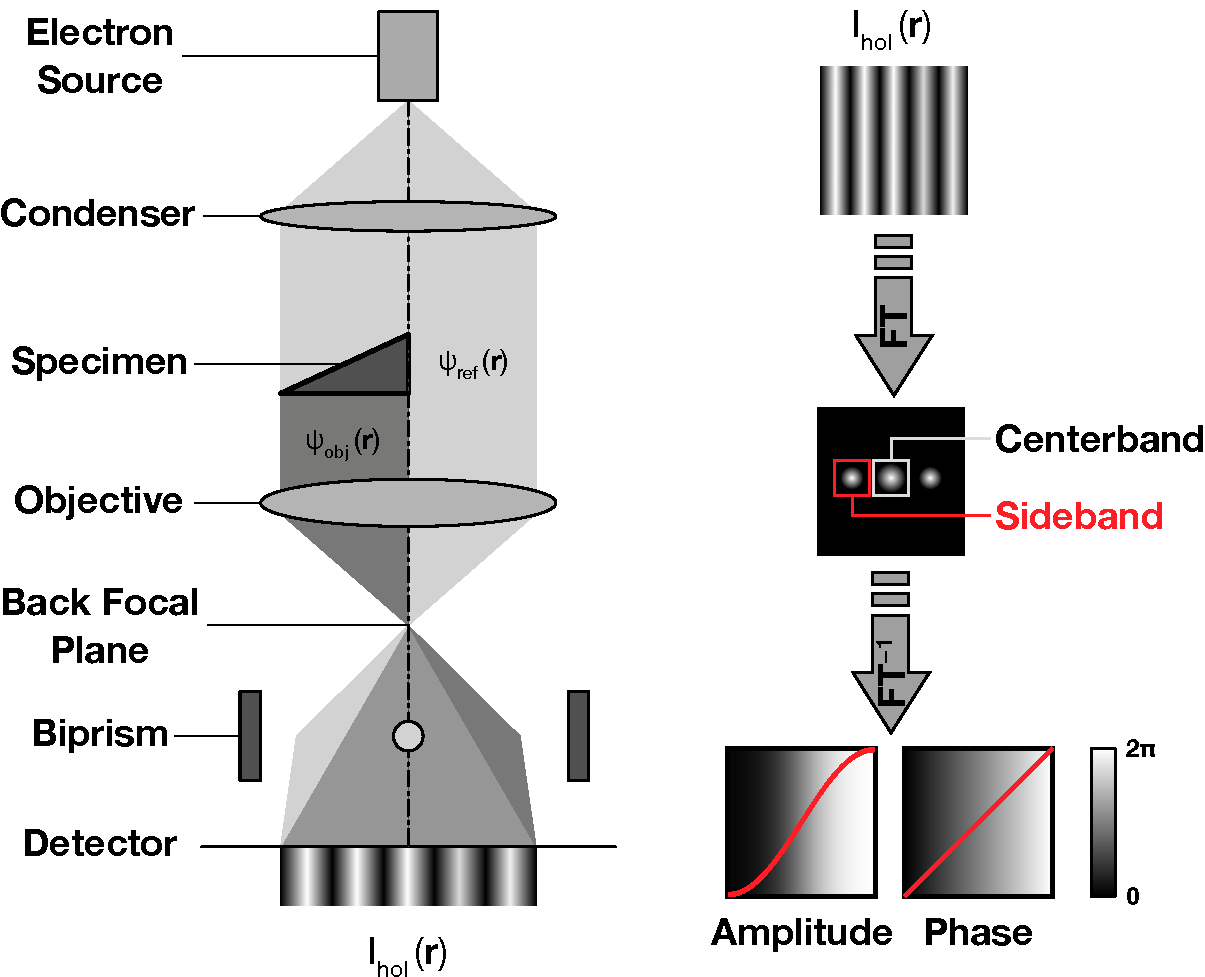
\includegraphics[width=0.8\textwidth]{Figures/Schematics/Theoretical Foundations/TEM-off-axis-holography-setup.pdf}
	\caption{\emph{Left:} Schematic illustration of the acquisition of an off-axis electron hologram in a TEM \cite{Lehmann1994,Voelkl1995,Voelkl1999,Lehmann2002,Lichte2008}. Part of electron wave propagates through the specimen, resulting in the modulated object wave ${\psi}_{\mathit{obj}}\left(\vb{r}\right)$, while the other part propagates through a nearby vacuum region, resulting in the unmodulated reference wave ${\psi}_{\mathit{ref}}\left(\vb{r}\right)$, ultimately creating an interference pattern after being superimposed through the deflection of a biprism \cite{Moellenstedt1956,Lehmann1994,Voelkl1995,Voelkl1999,Lehmann2002,Lichte2008}. \emph{Right:} Schematic illustration describing the reconstruction process of an off-axis electron hologram \cite{Lehmann1994,Voelkl1995,Voelkl1999,Lehmann2002,Lichte2008}. After the interference pattern is Fourier transformed, resulting in a centerband and two sidebands $\left(\pm 1\right)$, one of the two sidebands is inversely Fourier transformed, yielding the amplitude $a\left(\vb{r}\right)$ and the phase $\varphi\left(\vb{r}\right)$ (with their profiles indicated by the red curves) \cite{Lehmann1994,Voelkl1995,Voelkl1999,Lehmann2002,Lichte2008}.}
	\label{fig:TEM-off-axis-holography-setup}
\end{figure}
By coherently overlapping both electron waves under an angle $\beta$ through the deflection of a so called Möllenstedt biprism \cite{Moellenstedt1956}, the desired hologram can be obtained:
\begin{equation}
	I_{\mathit{hol}}\left(\vb{r}\right) = 1 + a^2\left(\vb{r}\right) + 2\mu a\left(\vb{r}\right)\cos(2\pi \vb{q}_c\vb{r} + \varphi\left(\vb{r}\right) + \theta\left(\vb{r},\vb{q}_c\right)),
\end{equation}
with the amplitude $a\left(\vb{r}\right)$ and the phase $\varphi\left(\vb{r}\right) = {\varphi}_{\mathit{obj}}\left(\vb{r}\right) - {\varphi}_{\mathit{ref}}\left(\vb{r}\right)$ of the reconstructed electron wave ${\psi}_{\mathit{el}}\left(\vb{r}\right)$, the carrier frequency of the interference fringes $\abs{\vb{q}_c} = {\beta}/{\lambda}$\footnote{For his introduction of the wavelength of particles $\lambda = h / p$ in 1924 \cite{BrogliePhD1924}, Louis~de~Broglie was awarded the Nobel~Prize in 1929 \cite{Broglie1929}.}, the corresponding contrast $\mu = \left(I_{\mathit{max}}\left(\vb{r}\right) - I_{\mathit{min}}\left(\vb{r}\right)\right) / \left(I_{\mathit{max}}\left(\vb{r}\right) + I_{\mathit{min}}\left(\vb{r}\right)\right)$ \cite{Voelkl1999,Lehmann2002,Lichte2008} and an additional phase modulation $\theta\left(\vb{r}, \vb{q}_c\right)$ \cite{LehmannPhD1997}. The resulting hologram therefore contains information about the amplitude in the form of contrast modulation and the phase in the form of interference fringe bending \cite{Voelkl1999,Lehmann2002,Lichte2008}.

The above mentioned distortion-induced phase modulations $\theta\left(\vb{r}, \vb{q}_c\right)$, representing the microscope's non-isoplanatic aberrations, make the recording of an empty hologram, where the specimen is removed and both the object and reference wave propagate through the vacuum region, directly after each object hologram necessary, allowing for the normalization of the amplitude and resulting in \cite{Voelkl1999,Lehmann2002,Lichte2008}:
\begin{equation}
  I_{\mathit{emp}}\left(\vb{r}\right) = 1 + 2\mu \cos(2\pi \vb{q}_c \vb{r} + \theta\left(\vb{r}, \vb{q}_c\right)).
\end{equation}
Being a two-step process, electron holography requires the subsequent numerical reconstruction of the recorded hologram \cite{Voelkl1999,Lehmann2002,Lichte2008}. For this purpose, the Fourier transform of the electron hologram can be calculated \cite{Lehmann1994,Voelkl1995,Voelkl1999,Lehmann2002,Lichte2008}:
	\begin{alignat}{3}
		\mathcal{F}\left\{ I_{\mathit{hol}}\left(\vb{r}\right) \right\} &= \mathcal{F}\left\{ 1 + a^2\left(\vb{r}\right) \right\} &\qquad\text{Centerband}& \notag \\
		&+ \mu \mathcal{F}\left\{ a\left(\vb{r}\right)e^{i\left(\varphi\left(\vb{r}\right) + \theta\left(\vb{r},\vb{q}_c\right)\right)} \right\} * \delta\left(\vb{q} - \vb{q}_c\right) &\quad\text{Sideband $\left(+1\right)$}& \notag \\
		&+ \mu \mathcal{F}\left\{ a\left(\vb{r}\right)e^{-i\left(\varphi\left(\vb{r}\right) + \theta\left(\vb{r},\vb{q}_c\right)\right)}\right\} * \delta\left(\vb{q} + \vb{q}_c\right) &\qquad\text{Sideband $\left(-1\right)$}&.
	\end{alignat}
Subsequently centering and isolating one\footnote{Usually the sideband in reference wave direction.} of the two sidebands and calculating the inverse Fourier transform $\mathcal{F}^{-1}$ results in the reconstructed electron wave (\cref{fig:TEM-off-axis-holography-setup}):
\begin{equation}
	{\psi}_{\mathit{el}}\left(\vb{r}\right) = \mu a\left(\vb{r}\right)e^{i\varphi\left(\vb{r}\right)},
\end{equation}
where the phase $\varphi\left(\vb{r}\right)$ is $2\pi$-wrapped to an interval of $\interval{-\pi}{\pi}$ \cite{Lehmann1994,Voelkl1995,Voelkl1999,Lehmann2002,Lichte2008}.

It should further be noted that although the reference wave is often assumed to be free from perturbations, various stray field effects in real-world experimental setups, especially in electrical biasing EH, necessitate shielding against these unwanted modulations \cite{Wagner2019,Wagner2022}.

\subsection{Electron Holography of the Electrostatic Potential} \label{ssec:electron-holography-electrostatic-potential}
The potential distribution of a specimen is encoded in its object hologram, where, in the absence of a magnetic vector potential, the object phase can derived from the Wentzel-Kramer-Brillouin approximation:
\begin{equation}
  \label{eq:electron-holography-electrostatic-potential}
  \varphi_{\mathit{obj}}\left(\vb{r}\right) = \frac{\pi}{\lambda E}\int\limits_{L} \phi\left(\vb{r}\right) \dd{z} = \sigma \phi_{\mathit{proj}}\left(\vb{r}\right),
\end{equation}
with a straight line integration path $L$ parallel to the $z$-axis (i.\,e.\ the electron beam direction), an acceleration voltage dependent interaction constant $\sigma = \pi / \lambda E$ and the projected electric potential $\phi_{\mathit{proj}}\left(\vb{r}\right)$ \cite{Voelkl1999,Lehmann2002,Lichte2008}. From this phase shift, the mean inner potential can be derived:
\begin{equation}
  \label{eq:electron-holography-MIP}
  \varphi_{\mathit{obj}}\left(\vb{r}\right) = \sigma \phi_{\mathit{MIP}}\left(\vb{r}\right) t
\end{equation}
with the intrinsic mean inner potential $\phi_{\mathit{MIP}}\left(\vb{r}\right)$, given by the electrostatic potential of the nuclei, and the specimen thickness $t$ \cite{Voelkl1999,Lehmann2002,Lichte2008}. This possibility to extract information about the electrostatic potential distribution in specimens, especially when the amplitude profile is unmodulated and offers no significant insight into the investigated specimen, makes electron holography an excellent method for in situ investigations of semiconductor nanodevices (i.\,e.\ electrical biasing electron holography) \cite{Tonomura1987,Lehmann2002,Lichte2008}, as described in the following \cref{ssec:electron-holography-pn-junctions}.
\subsection[Electron Holography of \texorpdfstring{$p$-$n$}{\textit{p}-\textit{n}}-Junctions]{Electron Holography of $\boldsymbol{p}$-$\boldsymbol{n}$-Junctions} \label{ssec:electron-holography-pn-junctions}
Based on \cref{eq:electron-holography-electrostatic-potential,eq:electron-holography-MIP}, the phase shift of a $p$-$n$-junction is given by:
\begin{equation}
  \label{eq:EH-phase-shift-specimen}
  \varphi\left(\vb{r}, U_{\mathit{ext}}\right) = \sigma \left[\phi_{\mathit{MIP}}\left(\vb{r}\right)\left(t_{\mathit{act}} + 2t_0\right) + \phi_{\mathit{pn}}\left(\vb{r}, U_{\mathit{ext}}\right)t_{\mathit{act}}\right],
\end{equation}
with the electrostatic potential of the $p$-$n$-junction $\phi_{\mathit{pn}}\left(\vb{r}, U_{\mathit{ext}}\right)$ and the specimen thickness $t$, which is made up of an electrically inactive\footnote{Recent investigations have shown that the electrically inactive boundary layer across the specimen does indeed contribute to the measured phase shift \cite{Wagner2022}.} boundary layer $t_0$ and an electrically active layer $t_{\mathit{act}}$ \cite{Frabboni1987,Twitchett2002,Cooper2006,Cooper2007,Cooper2009,He2013,Yazdi2015}. Using the electrostatic potential, and by that extent the phase shift obtained through electron holography, the electric field $E_{\mathit{pn}}\left(r, U_{\mathit{ext}}\right)$ and charge carrier density $\rho\left(r, U_{\mathit{ext}}\right)$ can be derived using Poisson's equation \cite{Frabboni1987,Twitchett2002,Yazdi2015}.

As described in \cref{ssec:band-structure-p-n-junctions}, the electric properties of a $p$-$n$-junction, such as the phase jump (or potential step) $\Delta \varphi_{\mathit{pn}}\left(U_{\mathit{ext}}\right)$, depend on the applied bias $U_{\mathit{ext}}$, with electric stray fields below and above the specimen leading to an additional phase shift that extend into the vacuum reference region \cite{Frabboni1987,Twitchett2002,Yazdi2015}.

The above detailed description of the electrostatic potential assumes a constant distribution in $z$-direction (i.\,e.\ the electron beam direction), which is often not the case for real-world measurements \cite{Twitchett-Harrison2007,Wagner2019}. Electron tomography, being a projective measurement method, is able to resolve this additional information in $z$-direction, as detailed in the following \cref{sec:electron-tomography}.

\section{Electron Tomography} \label{sec:electron-tomography}
Tomographic reconstruction is an imaging method that uses $k$ $\left(n - 1\right)$-dimensional projections of an object of interest to create a $n$-dimensional map \cite{Ramm1996,Herman2009,Kuchment2014}. The mathematical foundation for tomographic reconstructions was given by Johann Karl August Radon in 1917 \cite{Radon1917}, after whom the corresponding (inverse) Radon transform is named.

Given a 2D function $f\left(x, z\right)$, the integral along the path $L$ is given by:
\begin{equation}
  \label{eq:2D-radon-transform}
  \hat{f}_{\alpha} \left(x\right) = \int \limits_{L} f\left(x, z\right) \dd{z},
\end{equation}
where $\alpha$ describes the direction along which the path $L$ runs parallel to the $z$-axis (i.\,e.\ the electron beam direction) \cite{Ramm1996,Herman2009,Kuchment2014}. This continuous accumulation of 1D~projections towards a 2D~function $\hat{f}\left(\alpha, l\right)$ (i.\,e.\ the Radon transform) yields the so called sinogram \cite{Ramm1996,Herman2009,Kuchment2014}.

The projection-slice theorem further states that the $\left(n - 1\right)$-dimensional projection of a $n$-dimensional function in real space corresponds to a $\left(n - 1\right)$-dimensional cut through the origin of the $n$-dimensional Fourier transform in Fourier space:
\begin{equation}
  \hat{F}_{\vb{\xi}} \left(g\right) = \iint \limits_{-\infty}^{+\infty} F\left(\vb{\hat{g}'}\right) \delta \left(\vb{\hat{g}'} - g \vb{\hat{\xi}}\right) \dd[2]{g'},
\end{equation}
where $F\left(\vb{\hat{g}'}\right)$ is the 2D~Fourier transform of the 1D~function $f\left(\hat{\vb{r}}\right)$ and $\hat{\vb{\xi}} = \left[\cos\left(\alpha\right), \sin\left(\alpha\right)\right]^\intercal$ \cite{Ramm1996,Herman2009,Kuchment2014}.

The reconstruction of the original image from the sinogram constitutes an inverse problem \cite{Ramm1996,Herman2009,Kuchment2014}. Given infinite angular resolution, an inverse Radon transform of the sinogram yields a perfect reconstruction that is identical to the original image \cite{Ramm1996,Herman2009,Kuchment2014}. Since infinite resolution is not feasible with current experimental methods, various reconstruction approaches have been developed over the years \cite{Ramm1996,Herman2009,Kuchment2014}. One of the most common techniques is the so called filtered (or weighted) back-projection, where each 1D~projection is back-projection against its projection direction and summed up:
\begin{equation}
  \tilde{F}\left(\vb{\hat{g}}\right) = \iint \limits_{-\infty}^{+\infty} F\left(\vb{\hat{g}'}\right) \delta \left(\vb{\hat{g}'} - g \vb{\hat{\xi}}\right) \dd{\vb{\hat{\xi}}} \dd[2]{g'} = \frac{F\left(\vb{\hat{g}}\right)}{\lvert g \rvert},
\end{equation}
where $\lvert g \rvert$ is the weighting filter caused by the overemphasis on low spatial frequencies in Fourier space \cite{Ramm1996,Herman2009,Kuchment2014}. This improper weighting of low spacial frequencies can be partially compensated for by a suitable filter (e.\,g.\ ramp, Hann, Gaussian), lessening the observed smearing in the reconstructed image \cite{Ramm1996,Herman2009,Kuchment2014}.

An alternative approach is the iterative reconstruction, where an algorithm starts with an assumed image and tries to minimize the difference between the current computed reconstruction and the original image \cite{Ramm1996,Herman2009,Kuchment2014}. This approach, while sometimes more accurate, is usually computationally more expensive \cite{Ramm1996,Herman2009,Kuchment2014}.

Further limitations arise not only from a limited angular range that is smaller than the ideal $\alpha = \pm \SI{90}{\degree}$ (i.\,e.\ missing wedge) \cite{Ramm1996,Herman2009,Kuchment2014}, but also from a detector that captures an region of interest smaller than the entire object (i.\,e.\ interior radon transform) \cite{Maass1992,Pan2005,DaSilva2018}.

In a TEM, the 2D~projections of the 3D~specimen are given by the electron beam propagating through the specimen towards the detector, where recent developments have demonstrated electron tomography with atomic spacial resolution \cite{Scott2012,Miao2016,Yang2017}. In detail, the 2D~phase shift of a 3D~potential distribution for a constant tilt angle $\alpha$ is given according to \cref{eq:electrostatic-poisson-green} \cite{Wolf2014,Lubk2014}:
\begin{equation}
  \varphi_{\mathit{obj}}\left(\vb{r}, \alpha \right) = \sigma \int\limits_{L\left(\alpha\right)} \phi\left(\vb{r}\right) \dd{z}.
\end{equation}
